\documentclass[a4paper,11pt]{article}
\usepackage[utf8]{inputenc}
\usepackage{geometry}
\geometry{left = 4.0cm, right = 4.0cm, top = 4.0cm, bottom = 3.5cm}
\usepackage[onehalfspacing]{setspace} 
\usepackage{graphicx}
\usepackage{tabularx}
\usepackage{hyperref}
\usepackage{float} 
\usepackage{ragged2e}
\usepackage{biblatex} 
\usepackage{listings}
\usepackage{xcolor}

\lstset{
  basicstyle=\ttfamily\footnotesize, % Typewriter font
  keywordstyle=\color{blue},         % Keywords in blue
  commentstyle=\color{gray},         % Comments in gray
  stringstyle=\color{red},           % Strings in red
  breaklines=true,                    % Wrap long lines
  numbers=left,                       % Line numbers on the left
  numberstyle=\tiny\color{gray},      % Line number styling
  frame=single,                       % Box around code
}

\addbibresource{literatur.bib}
\setlength{\bibitemsep}{1em}

\title{Chat Application Project Report}
\author{Hussein Hafid, Jan Rahimi, Mohamad Alzein, Zakaria}
\date{March 6, 2025}

\begin{document}
\justifying
\pagenumbering{Roman}

\maketitle

\section*{Course}
Object-Oriented Applications (DAT055)

\section*{Repository Link}
 [link placeholder]

\newpage
\tableofcontents
\newpage
\listoffigures
\newpage
\listoftables
\newpage

\section{Introduction}
\subsection{Project Requirements}
\subsection{Scope of the Application}
\subsection{CRC Cards}

\section{Design of the Chat Application}
\subsection{Overview of Software Architecture}
\subsection{Server-Side Design}
\subsubsection{Data Storage and Management}
\subsubsection{Server TCP Communication}
\subsection{Client-Side Design}
\subsubsection{Client Authentication}
\subsubsection{Client TCP Communication}
\subsubsection{Client Interaction and User Interface}
\subsection{Class Design with CRC Cards}

\section{Running the Application}
\subsection{System Requirements}
\subsection{Prerequisites}
\subsection{Installation}
\subsection{Usage}
\subsubsection{User Login}
\subsubsection{User Registration}
\subsubsection{The Main View}
\subsubsection{Searching for Chat Rooms}
\subsubsection{Joining Chat Rooms}
\subsubsection{Connecting to Chat Rooms}
\subsubsection{Sending and Receiving Messages}

\section{Discussion}
\subsection{Development Workflow}
\subsection{Challenges and Difficulties}
\subsection{Limitations}
\subsection{Conclusion}
\subsection{Future Improvements and Enhancements}

\newpage
\section{Sample Code}
\begin{lstlisting}[language=Java, caption=Example Code]
public class ChatClient {
    private Socket socket;
    private BufferedReader input;
    private PrintWriter output;

    public ChatClient(String serverAddress, int port) throws IOException {
        socket = new Socket(serverAddress, port);
        input = new BufferedReader(new InputStreamReader(socket.getInputStream()));
        output = new PrintWriter(socket.getOutputStream(), true);
    }

    public void sendMessage(String message) {
        output.println(message);
    }
}
\end{lstlisting}
\begin{figure}[h]\centering\caption{Java Code Example - Chat Client}\end{figure}

\newpage
\section{Sample UML Diagram}
\begin{figure}[h]
    \centering
    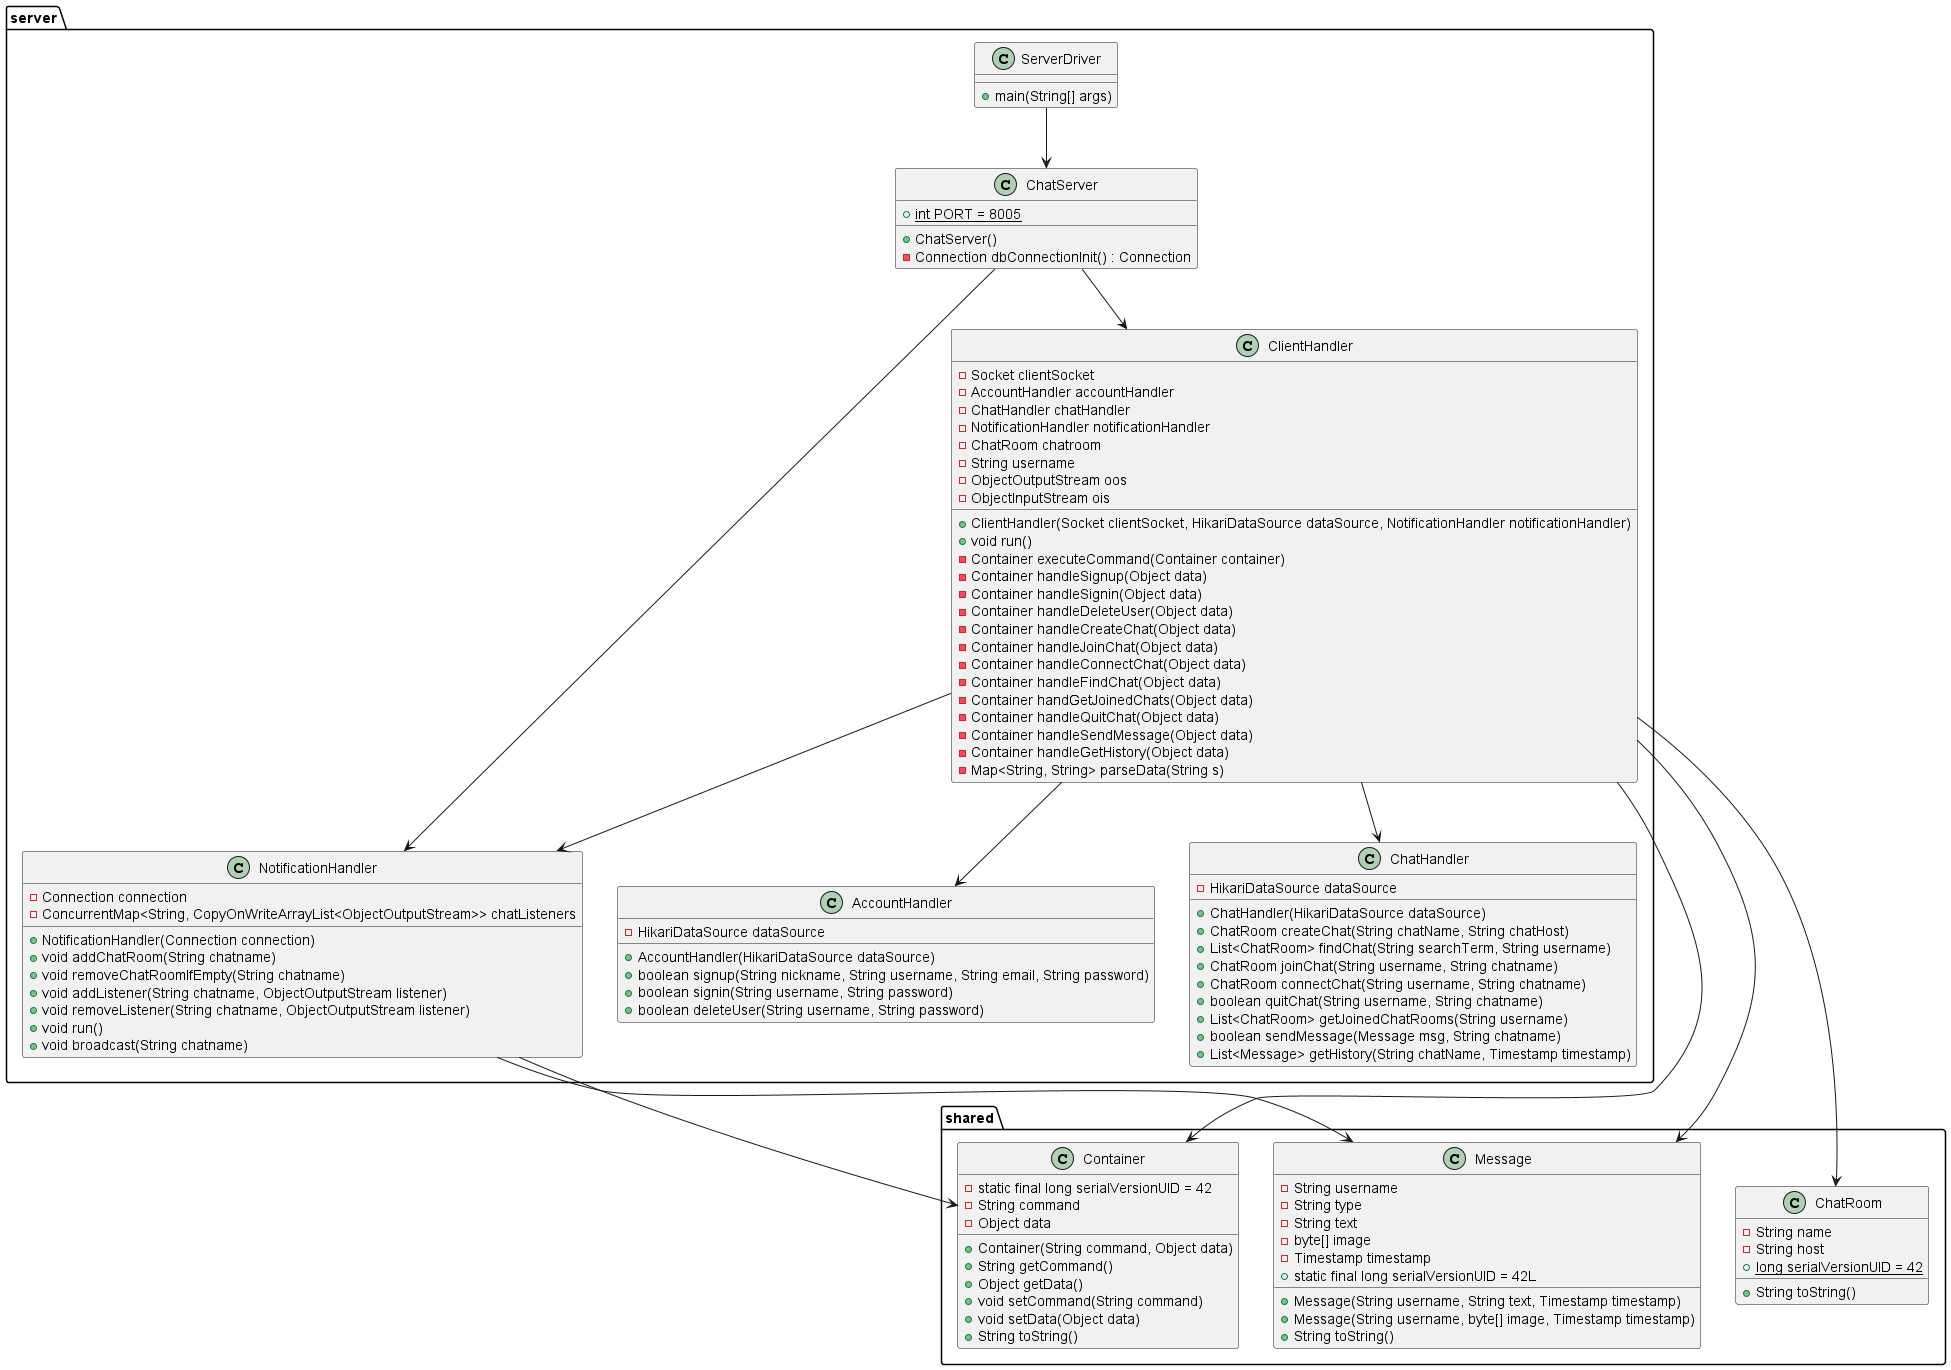
\includegraphics[width=0.8\textwidth]{server.png} % Change to your actual UML diagram file
    \caption{UML Diagram - Chat Client}
\end{figure}

\newpage
\pagenumbering{Roman}
\setcounter{page}{5}
\renewcommand\refname{References}
\addcontentsline{toc}{section}{References}
\printbibliography

\end{document}
